\documentclass[12pt]{article}
\usepackage[utf8]{inputenc}
\usepackage{amsmath, amssymb}
\usepackage{graphicx}
\usepackage{float}
\usepackage{booktabs}
\usepackage{geometry}
\usepackage{hyperref}
\usepackage{natbib}
\usepackage{caption}
\usepackage{tikz}
\usetikzlibrary{positioning,calc}

\geometry{margin=1in}

\title{Titanic Bayes Analysis}

% Define TikZ styles globally 
\tikzset{
	variable/.style={circle, draw, semithick, minimum size=1cm, inner sep=2pt},
	arrow/.style={->, semithick}
}

\begin{document}
	
	\maketitle
	
	\section{Titanic Causal Model}
	This project aims to estimate the effect of Age, Class, and Sex on the survival chance of the Titanic. 
	
	\subsection{Data description}
	The Titanic dataset is provided by the \texttt{causaldata} package and contains 2201 observations. 
	Variables include Age, Sex, Class, and Survival. 
	Age is binary: 1 = child, 2 = adult. 
	Sex is binary: 0 = woman, 1 = man. 
	Class has 4 categories (1–4). 
	Survival is binary: 0 = not survived, 1 = survived. 
	
	\section{Causal Models}
	The first causal model that aims to determine the direct effect of age on the survival chance is the following:
	
\begin{figure}[H]
	\centering
		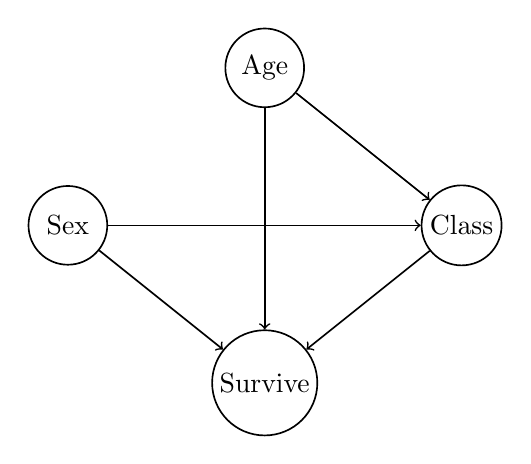
\begin{tikzpicture}
			% plain node definitions 
			\node[circle,draw,semithick,minimum size=1cm,inner sep=2pt] (age) {Age};
			\node[circle,draw,semithick,minimum size=1cm,inner sep=2pt] (sex) at (-2.5,-2) {Sex};
			\node[circle,draw,semithick,minimum size=1cm,inner sep=2pt] (class) at ( 2.5,-2) {Class};
			\node[circle,draw,semithick,minimum size=1cm,inner sep=2pt] (survive) at (0,-4) {Survive};
			
			% arrows
			\draw[->,semithick] (age) -- (class);
			\draw[->,semithick] (age) -- (survive);
			\draw[->,semithick] (sex) -- (class);
			\draw[->,semithick] (sex) -- (survive);
			\draw[->,semithick] (class) -- (survive);
		\end{tikzpicture}
	\caption{Causal Model to estimate the direct effect of Age on Survival chance}
	\label{fig:titanic_dag}
\end{figure}


Biasing paths are open.
Minimal sufficient adjustment sets for estimating the direct effect of Age on Survive include stratification by Class and Sex\\


The second Causal Model aims to determine the direct effect of Class on Survival in this case the minimal adjustment sets for estimating the direct effect of Class in Survival include stratification by Age and Sex\\


The third Causal Model aims to determine the direct effect of Sex on Survival and the minimal adjustment set is stratification by Class and Age\\

\section{Generative Model for Titanic Simulation}

\subsection{Root Variables (Exogenous Causes)}
These are determined outside our model - nothing causes them:
\begin{align*}
	\text{Sex}_i &\sim \text{Bernoulli}(p_{\text{sex}}) \\
	\text{Age}_i &\sim \text{Bernoulli}(p_{\text{child}})
\end{align*}
Where: 
- $p_{\text{sex}}$ = probability of being female
- $p_{\text{child}}$ = probability of being a child (vs adult)

\subsection{Class Assignment (Mediating Variable)}
Class is caused by both Age and Sex. We use multinomial regression with 4th as reference category:
\begin{align*}
	\text{Class}_i &\sim \text{Categorical}(\mathbf{p}_i) \\
	\log\left(\frac{p_{1st}}{p_{4th}}\right) &= \alpha_{1st} + \beta_{1st}^{age} \times \text{Age}_i + \beta_{1st}^{sex} \times \text{Sex}_i \\
	\log\left(\frac{p_{2nd}}{p_{4th}}\right) &= \alpha_{2nd} + \beta_{2nd}^{age} \times \text{Age}_i + \beta_{2nd}^{sex} \times \text{Sex}_i \\
	\log\left(\frac{p_{3rd}}{p_{4th}}\right) &= \alpha_{3rd} + \beta_{3rd}^{age} \times \text{Age}_i + \beta_{3rd}^{sex} \times \text{Sex}_i
\end{align*}
Where:
- $\beta^{age}$ = effect of being child on log-odds of each class vs 4th
- $\beta^{sex}$ = effect of being female on log-odds of each class vs 4th

\subsubsection{Class Assumption}
Being a Woman and a Child gives you higher chance of being first class then being adult men 

\begin{align*}
	\log\left(\frac{p_{1st}}{p_{4th}}\right) &= -1.39 + 1.2 \times \text{Child}_i + 0.9 \times \text{Female}_i \\
	\log\left(\frac{p_{2nd}}{p_{4th}}\right) &= -0.98 + 0.8 \times \text{Child}_i + 0.6 \times \text{Female}_i \\
	\log\left(\frac{p_{3rd}}{p_{4th}}\right) &= -0.13 - 0.5 \times \text{Child}_i - 0.3 \times \text{Female}_i
\end{align*}

\subsection{Survival}
The assumption is that survival chance is affected by Age and Sex.Children's and females are the first one to evacuate.I assume that the higher the class the better chance of survival because of the priority of for the bouts 

$$\text{Survive}_i \sim \text{Bernoulli}(p_i)$$
$$\text{logit}(p_i) = \alpha + \beta_{\text{class}} \times \text{Class}_i + \beta_{\text{sex}} \times \text{Female}_i + \beta_{\text{age}} \times \text{Child}_i$$

Again we model with the assumption of being a female child in a first class gives you the best chances of survival:

$$\text{logit}(p_i) = -1.4 + 1.2 \times \text{1stClass}_i + 0.8 \times \text{2ndClass}_i + 0.4 \times \text{3rdClass}_i + 1.2 \times \text{Female}_i + 1.0 \times \text{Child}_i$$

\end{document}

